\subsection{Проектирование и разработка клиентской части программного средства}
\label{sec:design:client}

Задачи клиентской части приложения включают отображение пользовательского интерфейса и обработку действий пользователя.
Типичными этапами его проектирования являются следующие~\cite{application_architecture_guide}:

\begin{itemize}
  \item идентификация типа клиентской части приложения, которое удовлетворяет установленным требованиям.
  Осуществление данного этапа осуществлено в подразделе~\ref{sec:design:architecture};
  \item выбор технологии пользовательского интерфейса. Осуществляется на основе анализа требуемой для реализации
  функциональности;
  \item проектирование UI. Хорошей практикой является реализация модульности, а также принципа разделения 
  ответственности компонентов;
  \item определение стратегии и протоколов обмена информации между уровнями. Поскольку рассматриваемый уровень является
  самым верхним, а его протоколы связи с серверной частью приложения были рассмотрены в
  пункте~\ref{sec:design:server:protocols}, то данный вопрос считается решенным и рассматриваться не будет.
\end{itemize}

Ранее был проведен анализ и осуществлен выбор целевой платформы для реализации клиентской части приложения, был выбран
язык программирования. Однако, существует огромное число специализированных технологий и фреймворков по созданию
пользовательских интерфейсов. Представляется целесообразным провести уточнение средств разработки.

\subsubsection{} Уточнение выбора технологий программирования
\label{sec:design:client:technologies}

Одной из широко используемых в настоящее время библиотек по созданию интерактивных интерфейсов веб-приложения является
библиотека React. Выбор в ее пользу был осуществлен вследствие наличия опыта по ее использованию у членов команды.
Особенностями данной библиотеки являются следующие~\cite{habr_react_introduction}:

\begin{itemize}
  \item кроссплатформенность. Переиспользование существующего кода возможно даже на других платформах
  благодаря проекту React Native;
  \item декларативность: использование элементов (стандартных для React объектов, которые представляют собой HTML-теги)
  и компонентов (объекты, создаваемые разработчиком);
  \item JSX: техника создания и использования компонентов с помощью HTML-подобного синтаксиса, который применяется
  прямо в Javascript коде;
  \item виртуальный DOM: дерево React элементов, которое отрисовывается в браузере, причем изменения в нём не требуют
  полной перерисовки всего интерфейса. Позволяет значительно улучшить быстродействие при использовании библиотеки.
\end{itemize}

Строго говоря, использование JSX является опциональным и может как не использоваться при разработке с React, так и
использоваться при разработке с помощью других библиотек. Однако, он значительно упрощает исходный код компонентов.
Например, следующий React код

\begin{flushleft}
  \qquad\qquad\qquad return <div>Hello\{this.props.children\}</div>;
  \end{flushleft}
  после компиляции будет преобразован в следующий
  \begin{flushleft}
  \qquad\qquad\qquad return React.createElement(\\
  \qquad\qquad\qquad\qquad ``div'',\\
  \qquad\qquad\qquad\qquad null,\\
  \qquad\qquad\qquad\qquad ``Hello '',\\
  \qquad\qquad\qquad\qquad this.props.children\\
  \qquad\qquad\qquad );
\end{flushleft}

Лаконичность использования JSX очевидна. Некоторым кажется сомнительным данный подход, в котором смешивается
исполняемый код и код разметки. Однако, данное смешение формирует исходный код представления. Кроме того, в других
фреймворках используются специальные конструкции по реализации, например, циклов, условий, в то время как при
использовании JSX нужды в новых конструкциях нет, ведь используются стандартные операторы языка Javascript.

Одна из классификаций компонентов React предполагает их разделение на pure (простые) и stateful (имеющие внутреннее
состояние)~\cite{react}. Простые компоненты, реализованные в виде классов, унаследованных от\linebreak React.Component,
переопределяют метод render(), который принимает некоторый набор исходных данных и возвращает элемент,
предназначенный для отображения. Компоненты другого класса имеют внутри себя некоторые данные, образующие их состояние.
Чтобы React узнал, что данные изменились, и осуществил перерисовку измененных компонентов, требуется использовать
специальный метод this.setState(...). 

Для упрощения управления состоянием компонентов могут применяться различные техники. Одной из них является использование
специальной библиотеки Redux. Он предназначен для управления потоком данных и их связями. В React связь между двумя
компонентами, не имеющими отношения родитель-потомок (дочерний элемент), не рекомендуется. React обращает внимание,
что если такое сделать (создать связь), можно вполне создать собственную глобальную систему событий по шаблону Flux;
и именно в этот момент и появляется Redux.

С Redux у нас есть хранилище, в котором можно сохранять все состояния приложения. Если в компоненте A происходит
изменение состояния, оно затем передается в хранилище, а другие компоненты B и C, которые должны знать об этом
изменении состояния в компоненте A, могут получать эту самую информацию об этом изменении из хранилища.

Сравнение работы приведено на рисунке~\ref{fig:design:client:technologies:redux}

\begin{figure}[!ht]
	\centering
	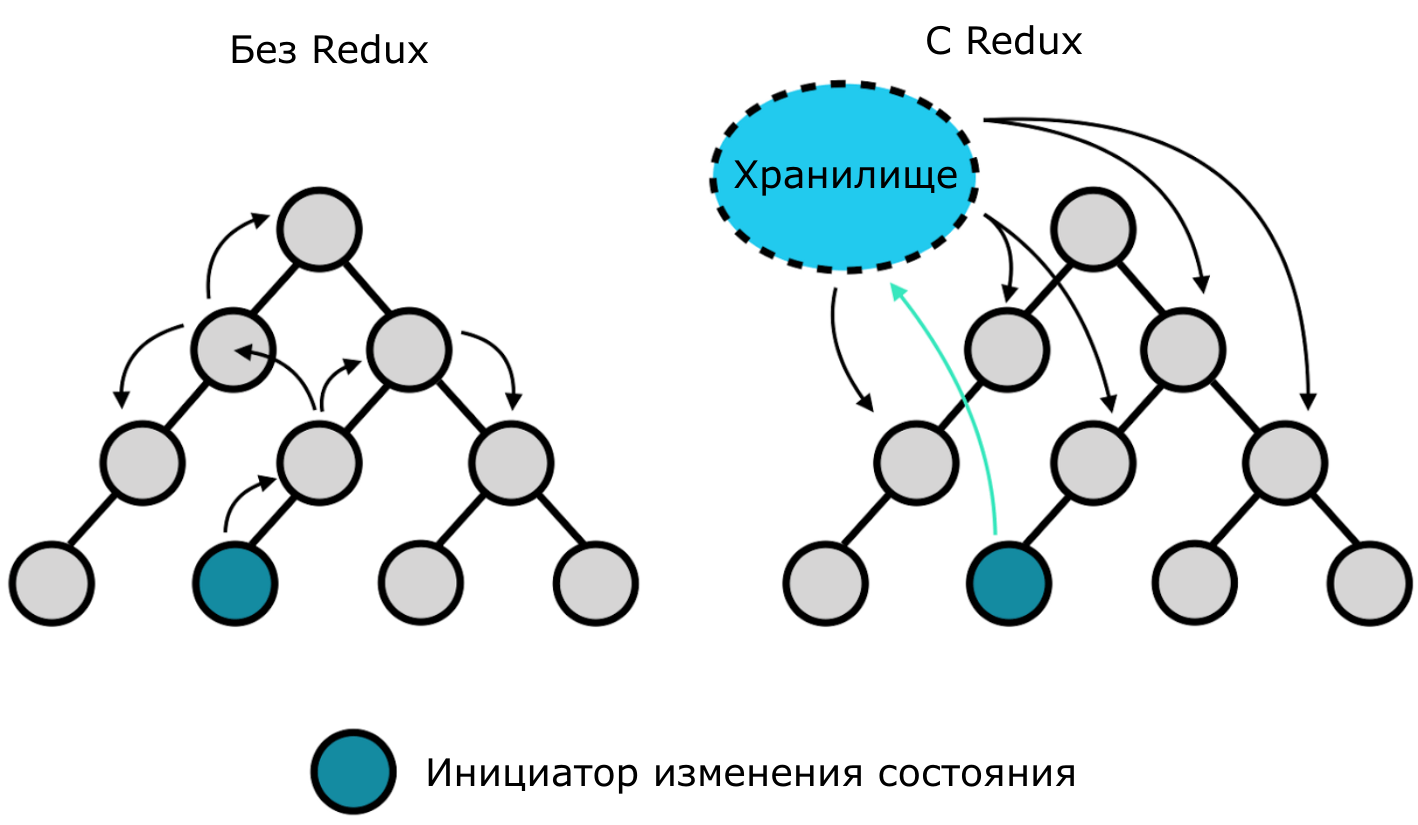
\includegraphics[scale=0.32]{redux.png} 
	\caption{Сравнение работы с Redux и без него}
	\label{fig:design:client:technologies:redux}
\end{figure}

Redux состоит из следующих составных частей:

\begin{itemize}
  \item действия(actions) -- Это просто события, созданные с помощью функций для отправки данных из приложения в
  хранилище. Данные могут быть отправлены различными способами, такими как отправка формы, вызов API или обычного
  взаимодействия с пользователем. Каждое действие в Redux имеет свойство type, которое описывает тип действия, а также
  «важную» информацию, отправляемую в хранилище;
  \item редюсеры (reducer). Поскольку Redux не позволяет приложению вносить изменения в состояния компонентов,
  сохраняемых в хранилище, он использует dispatch() для этого. Функция dispatch() просто указывает на намерение изменить
  данное состояние, но на самом деле не меняет его, вот почему и нужны редюсеры (Reducer).
  Редюсеры (Reducer) – это функции, которые считывают из хранилища текущее состояние приложения через отправленное
  действие, а затем возвращают новое состояние;
  \item хранилище похоже на сердце фреймворка Redux. Это единственный источник истины, в котором находятся все состояния
  приложения и который обеспечивает доступ к состоянию с помощью нескольких методов, действий отправки данных и
  регистрации записей. Любое отправленное действие возвращает новое состояние  данных в хранилище с помощью
  редюсеров~\cite{redux}.
\end{itemize}

Однако, Redux представляет собой только библиотеку. Ограничения на архитектуру приложения не накладываются, однако
сохраняется необходимость ее реализации программистом. Одним из вариантов является разбиение всех компонентов на
контейнерные и презентационные~\cite{presentational_and_container_components}. Особенности создания презентационных
компонентов следующие:

\begin{itemize}
	\item их задача заключается в определении, как должны выглядеть элементы;
	\item не зависят от других частей приложения;
	\item получают данные исключительно в качестве входных параметров;
	\item не изменяют данные;
	\item редко имеют собственное состояние (в таком случае это состояние UI, а не собственно данные);
	\item обычно содержат JSX разметку и имеют относящиеся к ним стили.
\end{itemize}

В это же время особенности контейнерных компонентов заключаются в следующем:

\begin{itemize}
	\item их задача заключается в определении, как элемент должны работать;
	\item предоставляют данные и методы их обработки другим компонентам;
	\item как правило имеют некоторые данные в виде состояния;
	\item обычно не содержат JSX разметки и никогда не имеют стилей.
\end{itemize}

Использование данного подхода имеет следующие преимущества:

\begin{itemize}
	\item достигается выполнение принципа разделения ответственности;
	\item появляется возможность легкого переиспользования компонентов с различными источниками данных;
	\item одни и те же презентационные компоненты могут использоваться повсеместно в приложении;
	\item презентационные компоненты формируют <<палитру>>. Их внешний вид может изменяться без влияния на логику приложения.
\end{itemize}

Еще один важный момент относительно проектирования UI, помимо содержания и интерактивных пользовательских
взаимодействий, касается стилизации внешнего вида компонентов. Существует несколько подходов по ее
исполнению~\cite{styling_react}: использование внутренних (inline) и внешних стилей.

Первый подход имеет множество недостатков:

\begin{itemize}
  \item невозможно использование медиа-запросы, чтобы, например, реагировать на изменения ширины экрана или отличать
  мобильное устройство от настольного компьютера;
	\item невозможно использование псевдоклассов и псевдоэлементов, например: :hover, :active, :before, :after;
	\item значительное увеличение размера разметки и снижение производительности;
	\item невозможно переопределение стилей по более сложным селекторам.
\end{itemize}

Тем не менее, Facebook, как компания разработчик React, несмотря на описанные недостатки, выступает за использование
inline стилей. Причиной этому является стремление обеспечить единообразие с React Native, поскольку там возможность
стилизации обеспечивается только данным подходом.

Второй подход -- использование внешних стилей -- является более традиционным для веб-разработки. Его эволюционное
развитие включает несколько этапов:

\begin{itemize}
  \item cоздание одного файла .css со стилями, который подключается один раз глобально в главный html файл. В React
  компонентах используется тег className со значениями имен классов из этого файла;
  \item hазбиение единого файла стилей на множество файлов в соответствии с реализованными компонентами. В файлы
  компонентов подключаются лишь те стили, которые там необходимы. Преимущества данного подхода заключаются в простоте
  поиска файла, в который необходимо внести изменения, и в простоте удаления компонентов и соответствующих им файлов стилей;
	\item использование различных препроцессоров стилей, таких как\linebreak SASS/SCSS, LESS и прочих.
\end{itemize}

Использование SASS по сравнению с обычным CSS предоставляет следующие преимущества~\cite{sass_guide}:

\begin{itemize}
	\item переменные, в которых можно хранить значения цветов, шрифтов, а также любые другие значения;
	\item вложенность, что приводит к большей наглядности файлов стилевых таблиц за счет соответствия иерархии HTML кода;
	\item фрагментирование, то есть обеспечение модульности;
  \item импортирование других файлов стилей, которое, в отличие от CSS, вместо создания новых HTTP запросов подставляет
  указанный файл в тот, где он вызывается, таким образом на выходе получается единственный файл стилей;
	\item примеси (mixins), которые представляют собой группы деклараций, используемые по нескольку раз;
	\item наследование, позволяющее привносить наборы свойств от одного селектора к другому;
	\item использование математических операторов.
\end{itemize}

Таким образом, на основании проведенного уточнения технологий для использования выбираем следующие:
React в связке с Redux и SCSS, кроме того, для разметки в коде повсеместно будет использоваться JSX.

\subsubsection{} Проектирование клиентской части приложения
\label{sec:design:client:ux}

Далее рассмотрим вопрос взаимодействия пользователя с клиентской частью приложения. Известно, что удобство пользования
программным средством может во многом определять успешность проекта в целом~\cite{code_complete}.

Схема работы клиентской части программной системы представлена на рисунке~\ref{fig:design:client:ux:client_algorithm}.
Среди ее особенностей можно выделить в высокой степени соответствие диаграмме прецедентов, которая была составлена и
рассмотрена в пункте~\ref{sec:domain:model:use_cases}. Кроме того, данный чертеж представляет собой отображение чертежа
схемы серверной части с отличием в том, что там делается акцент на взаимодействие с базой данных, а в данном чертеже --
на отображении данных и интерактивном взаимодействии с пользователем.

\begin{sidewaysfigure}
  \centering
    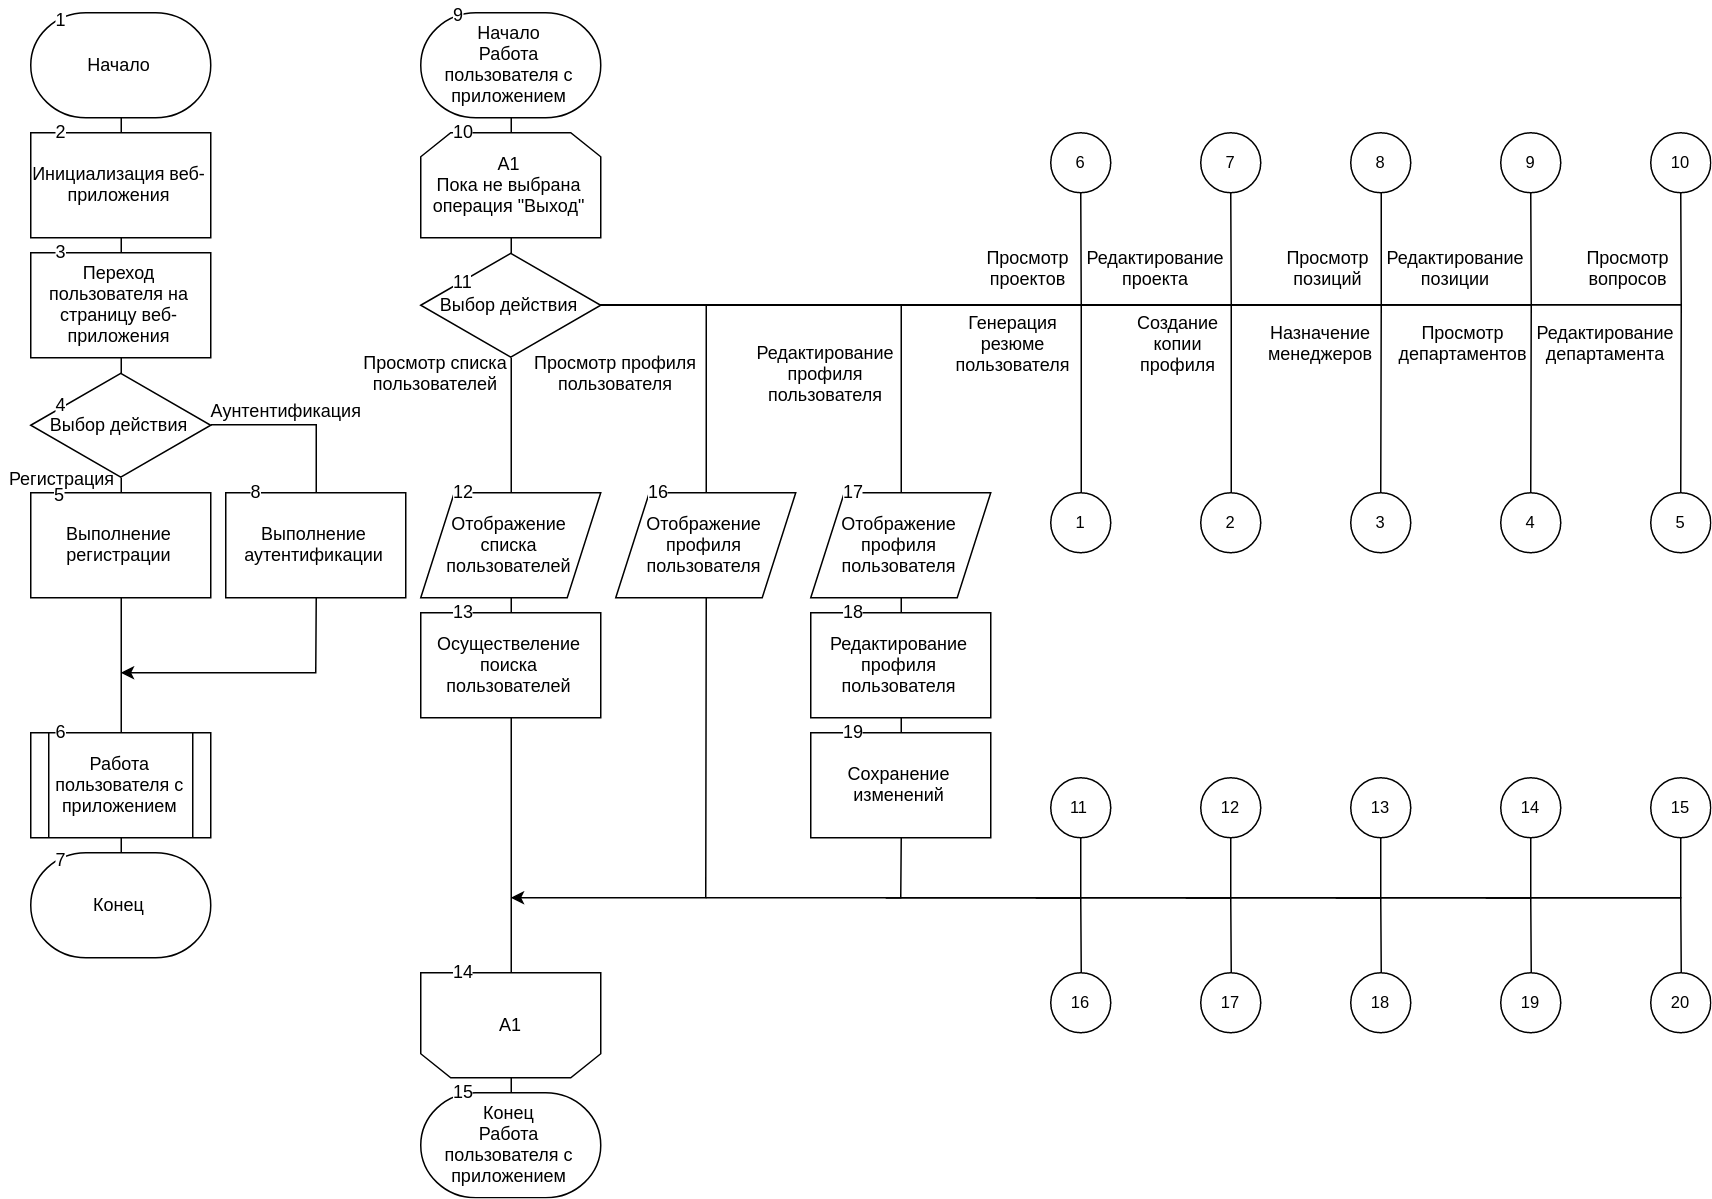
\includegraphics[scale=0.37]{client-algorithm-1.png}
    \caption{Схема программы клиентской части программного средства}
    \label{fig:design:client:ux:client_algorithm}
  \end{sidewaysfigure}
  
  \begin{sidewaysfigure}
  \ContinuedFloat
  \centering
    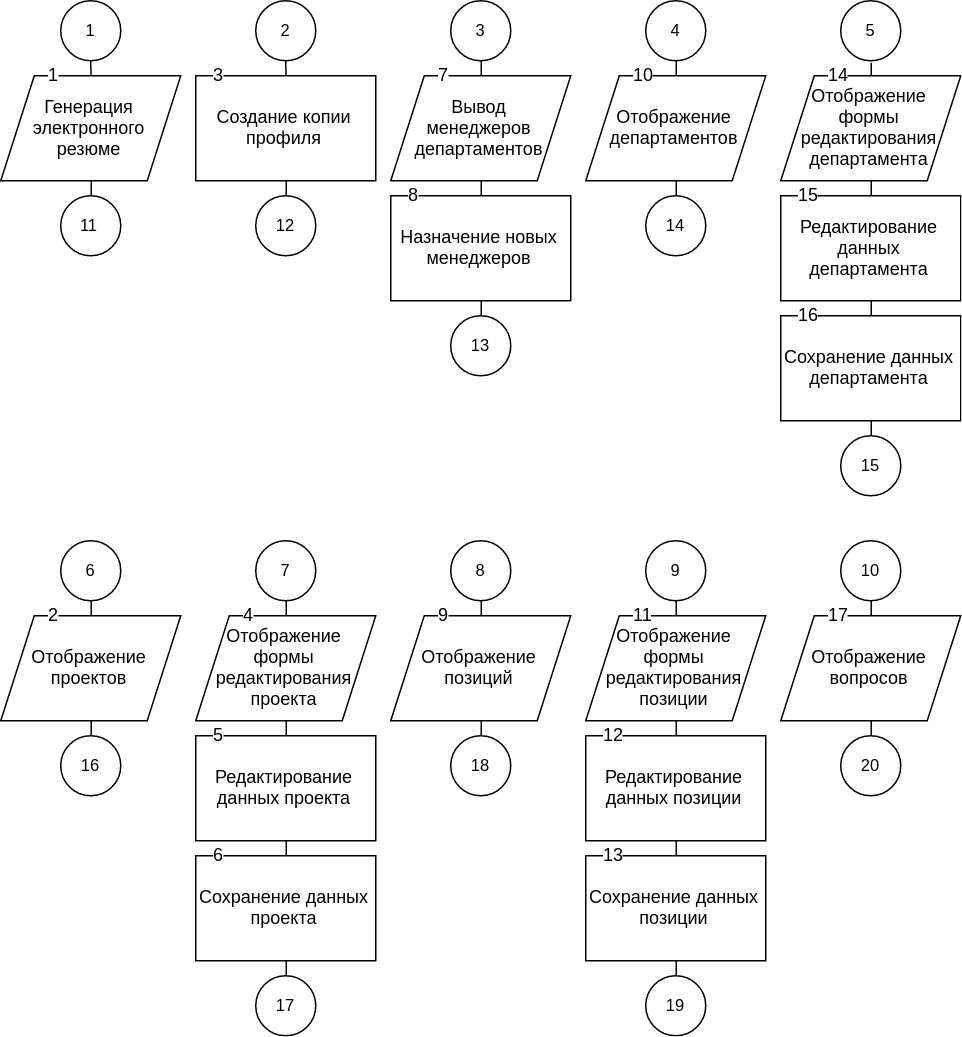
\includegraphics[scale=0.4]{client-algorithm-2.png}
    \caption{Схема программы клиентской части программного средства (окончание)}
  \end{sidewaysfigure}

Таким образом, составленная схема клиентской части ПС будет использована при разработке навигации (routing) по
страницам веб-приложе\-ния.

\subsubsection{} Конструирование клиентской части приложения
\label{sec:design:client:development}

Наконец, по завершению этапов проектирования и подготовки можно приступить к собственно созданию исходных кодов
приложения. Ключевые фрагменты кода, описание которых приведено в данном пункте, приведены в приложении А.

Для начала необходимо создать корневой файл index.html. Ключевая его особенность состоит в следующем теге
\begin{flushleft}
\qquad\qquad\qquad\qquad\qquad <div id=``root''></div>
\end{flushleft}

Несмотря на то, что он объявляется пустым, именно в него библиотека React подставит всё приложение.

Кроме этого, в данном файле подключается основная зависимость приложения -- непосредственно сама библиотека React и
библиотека по управлению виртуальным деревом элементов браузера, а также пакет bun\-dle.js, в который будет собран весь
созданный исходный код. Помимо библиотек, подключаются некоторые файлы стилей, необходимые для корректной работы
некоторых компонентов, например, специальных шрифтов, предоставляющих возможность использования большого количества
специальных иконок.

Алгоритм генерации резюме пользователя представлен на рисунке~\ref{fig:design:client:ux:resume_generate}.

\begin{figure}[!h]
  \centering
    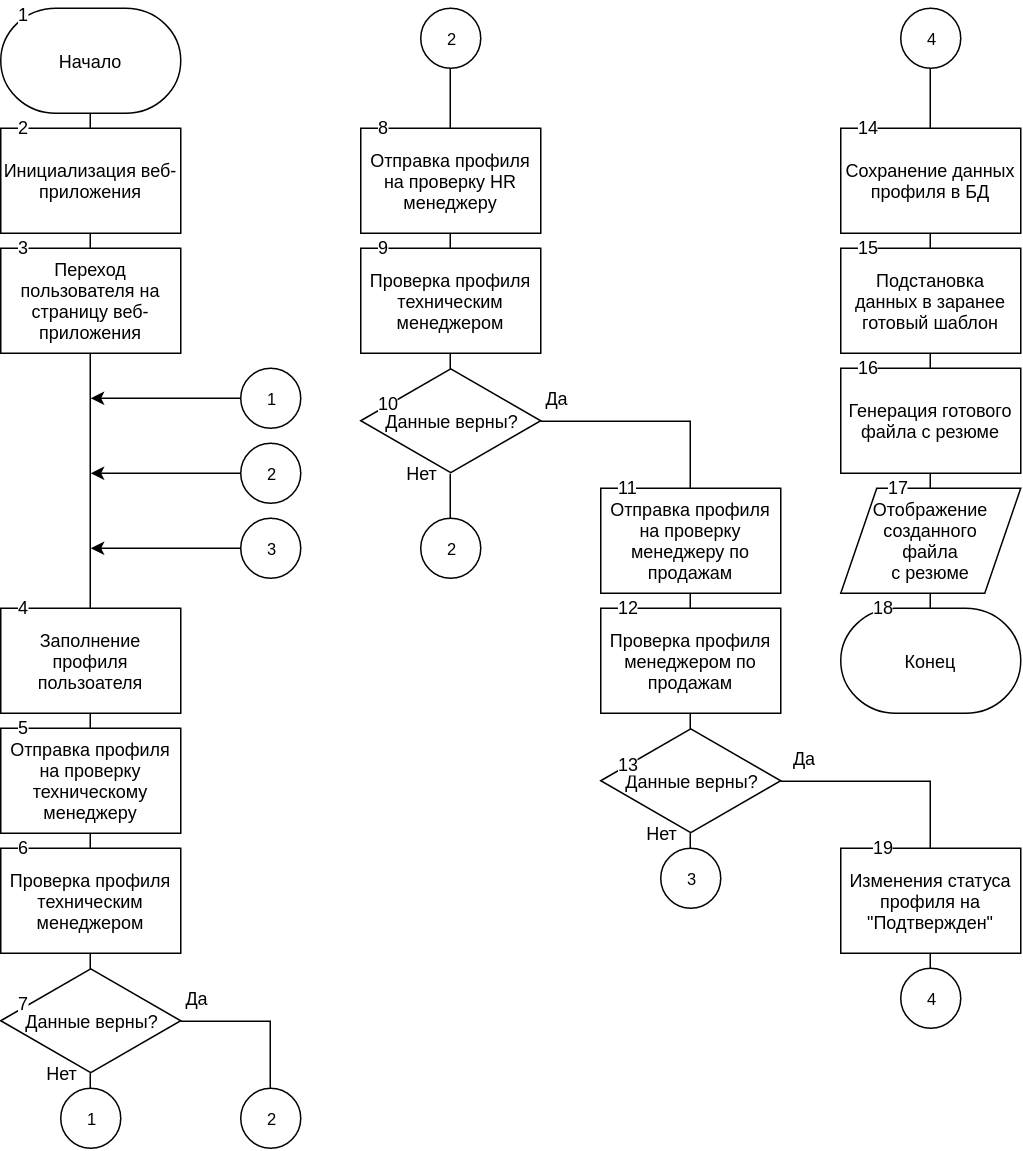
\includegraphics[scale=0.43]{resume-generate.png}
    \caption{Алгоритм генерации резюме пользователя}
    \label{fig:design:client:ux:resume_generate}
\end{figure}
